\documentclass[11pt]{article}
\usepackage[margin=1in]{geometry}
\usepackage{graphicx,booktabs,amsmath,xcolor,hyperref,float}
\newcommand{\todo}[1]{\textcolor{red}{[TODO: #1]}}
\newcommand{\needcite}{\textcolor{red}{\textsuperscript{[cite]}}}
\title{Multi-View Agreement as a Training-Free Reliability Signal\\for Selective Prediction in Medical VQA}
\author{\todo{authors and affiliations}}
\date{}
\begin{document}
\maketitle

\begin{abstract}
Medical visual question answering (VQA) models give fluent answers even when they are wrong. We study a training-free pipeline that wraps a vision-language model (Qwen/Qwen2.5-VL-7B-Instruct) and asks it the same question about several views of the image: the full image, a crop around a region the model itself localizes, a shifted crop, a random crop and an image with the region masked out. We test whether switching answers based on these views improves accuracy, and whether agreement between views tells us which answers to withhold. On the VQA-RAD test split ($n=451$), switching answers does not improve over the direct answer (direct accuracy 0.554 [0.508, 0.601]). Abstaining with a logistic regression over view-agreement features, with all weights and the threshold fixed on 500 training-split questions, answers 80.9\% of questions at accuracy 0.625 (+0.070 over answering everything, 95\% CI [0.046, 0.095]). The signal ranks answers better than plain confidence (AUROC 0.732 vs 0.666, difference 95\% CI [0.028, 0.103]), but this advantage does not persist within question types, so part of it reflects question difficulty. We report the limits of the approach, including that every test question was seen in earlier exploratory work.
\end{abstract}

\section{Introduction}
Clinicians need a model to say when it does not know. In medical VQA, a wrong answer delivered confidently can be worse than no answer.\needcite{} Selective prediction, where a model answers only when a reliability score is high enough, addresses this directly.\needcite{} Existing reliability scores for vision-language models are often built from the model's own confidence or from repeated sampling.\needcite{}

We ask a narrower question than ``can we make the model more accurate?'' We ask whether agreement between different views of the same image, obtained without any training, tells us which answers to trust. Our contributions are:
\begin{itemize}
\item A training-free pipeline that produces five answers per question from different views of the image, and a small set of agreement features computed from them.
\item A pre-specified evaluation protocol: decision rules, the scoring rule and the abstention threshold were fixed on a development set, locked by a hash of the configuration file, and applied once to the test split.
\item An honest account of the outcome. Switching answers does not help. Abstaining on the basis of view agreement helps, but a simple agreement score performs about as well as the fitted model, and the gain over confidence is concentrated where question types differ in difficulty.
\end{itemize}

\section{Related Work}
\todo{Add related work with real citations: medical VQA and VQA-RAD; selective prediction and risk--coverage analysis; confidence and consistency-based uncertainty for vision-language models; visual cropping and grounding for VLMs; hallucination in medical VLMs. No citations have been invented in this draft.}

\section{Method}
\paragraph{Views.} For each question the same VLM (Qwen/Qwen2.5-VL-7B-Instruct) is run on up to five inputs, all with the prompt suffix ``Answer concisely.'': (i) the full image (direct answer); (ii) a crop around a bounding box that the model itself predicts for the region relevant to the question, padded by 0.15 of the box and upsampled; (iii) a crop around a randomly shifted copy of that box (jitter fraction 0.10, seeded by question index); (iv) a crop of a random box of the same size as a control; (v) the full image with the predicted region masked out. A sixth call produces the box itself. \todo{state exactly how the confidence of an answer is computed in the pipeline, and how the region mask is applied.}

\paragraph{Agreement features.} Let $a_d, a_c, a_j, a_m, a_r$ be the normalized answers from the direct, crop, shifted-crop, masked and random-crop views, and $c$ the confidence of the direct answer. We use $c$ and five binary features: crop agrees with direct ($a_c=a_d$), shifted crop agrees with crop ($a_j=a_c$), masking changes the answer ($a_m\neq a_d$), shifted crop agrees with direct ($a_j=a_d$) and random crop agrees with direct ($a_r=a_d$).

\paragraph{Answer rule.} The final answer is chosen by a pre-set rule: switch from the direct answer to another rule only if it beats direct on the development set with McNemar $p<0.05$. No rule did, so the frozen answer is the direct answer.

\paragraph{Abstention.} The reliability score is the predicted probability of a logistic regression on the six features, fit on the development set to predict whether the direct answer is correct. The model abstains when the score is below the 20th percentile of development scores (target coverage 80.0\%), or when no valid box is produced. Table~\ref{tab:coef} lists the frozen weights.

\begin{table}[t]
\centering\small
\caption{Frozen logistic-regression weights (fit on the 500 development questions only).}\label{tab:coef}
\begin{tabular}{lr}
\toprule
Feature & Weight \\
\midrule
final\_conf & +2.345 \\
suff & +0.565 \\
stab & +0.676 \\
nec & -0.267 \\
jit\_agree & -0.128 \\
rand\_agree & +0.791 \\
intercept & -2.683 \\
abstention threshold (score) & 0.3075 \\
\bottomrule
\end{tabular}
\end{table}


\section{Experimental Setup}
\paragraph{Data.} The test set is the full VQA-RAD test split: 451 questions (251 yes/no, 200 open). The development set is 500 questions from the VQA-RAD training split. \todo{cite dataset; state license and how the images and questions were obtained.}
\paragraph{Scoring.} Strict scoring: yes/no answers are correct if the first word matches; open answers are correct on exact or whole-word match. An earlier, looser rule counted ``no'' inside ``normal'' as correct; on the development set the two rules agree on all 500 direct answers, but we use the strict rule throughout.
\paragraph{Statistics.} 95\% CIs are percentile bootstrap intervals over questions (2000 resamples). Answer rules are compared with McNemar's exact test. Selective accuracy at fixed coverage keeps the highest-scoring answers, with ties broken by confidence. Comparisons between signals use the same bootstrap resamples. The AUROC difference between the R2-VQA score and confidence is the pre-specified comparison; coverage-level comparisons are exploratory.
\paragraph{Protocol.} All decision rules, the scoring rule, and the abstention weights and threshold were fixed on the development set before the test split was run. The test run was executed once; the configuration file was locked by its hash, and the scoring step refuses to run if it changed.
\paragraph{Compute.} A single Colab T4 GPU. The pipeline uses six model calls per question; we report compute as calls per question because per-question wall-clock times were not logged.

\section{Results}
\subsection{Switching answers does not improve accuracy}
Direct accuracy on the test split is 0.554 [0.508, 0.601] (Table~\ref{tab:rules}, Figure~\ref{fig:bars}). No alternative answer rule beats it; the smallest $p$-value against direct is 0.111 and every rule has a lower point estimate. This matches the development set (Table~\ref{tab:dev}): cropping to the predicted region lowers accuracy from 0.520 to 0.478, and a crop at a random region of the same size gives 0.478 ($p=1.000$ against the predicted crop). The location of the predicted region therefore does not explain the crop answer.

\begin{table}[t]
\centering\small
\caption{Test accuracy of answer rules (VQA-RAD test, $n=451$, strict scoring, 95\% bootstrap CIs). Column 3 is gains/losses against direct; $p$ is McNemar's test.}\label{tab:rules}
\begin{tabular}{lccc}
\toprule
Answer rule & Accuracy [95\% CI] & Gain/loss & $p$ \\
\midrule
direct & 0.554 [0.508, 0.601] & 0/0 & -- \\
always\_crop & 0.525 [0.481, 0.572] & 22/35 & 0.111 \\
week6 rule (2 of 3 checks) & 0.550 [0.503, 0.596] & 5/7 & 0.774 \\
majority vote (direct, crop, shifted crop) & 0.543 [0.499, 0.590] & 19/24 & 0.542 \\
\bottomrule
\end{tabular}
\end{table}

\begin{table}[t]
\centering\small
\caption{Development set ablation (500 training-split questions, one session, strict scoring). Columns 3 and 4 count questions where the view is right and direct is wrong, and the reverse; $p$ is McNemar's test against direct.}\label{tab:dev}
\begin{tabular}{lrrrr}
\toprule
View & Accuracy & Gains & Losses & $p$ \\
\midrule
Direct answer (full image) & 0.520 & 0 & 0 & -- \\
Crop at predicted region & 0.478 & 18 & 39 & 0.008 \\
Crop at random region (same size) & 0.478 & 19 & 40 & 0.009 \\
Crop at shifted region & 0.464 & 20 & 48 & $<0.001$ \\
Predicted region masked out & 0.410 & 16 & 71 & $<0.001$ \\
\bottomrule
\end{tabular}
\end{table}


\begin{figure}[t]\centering
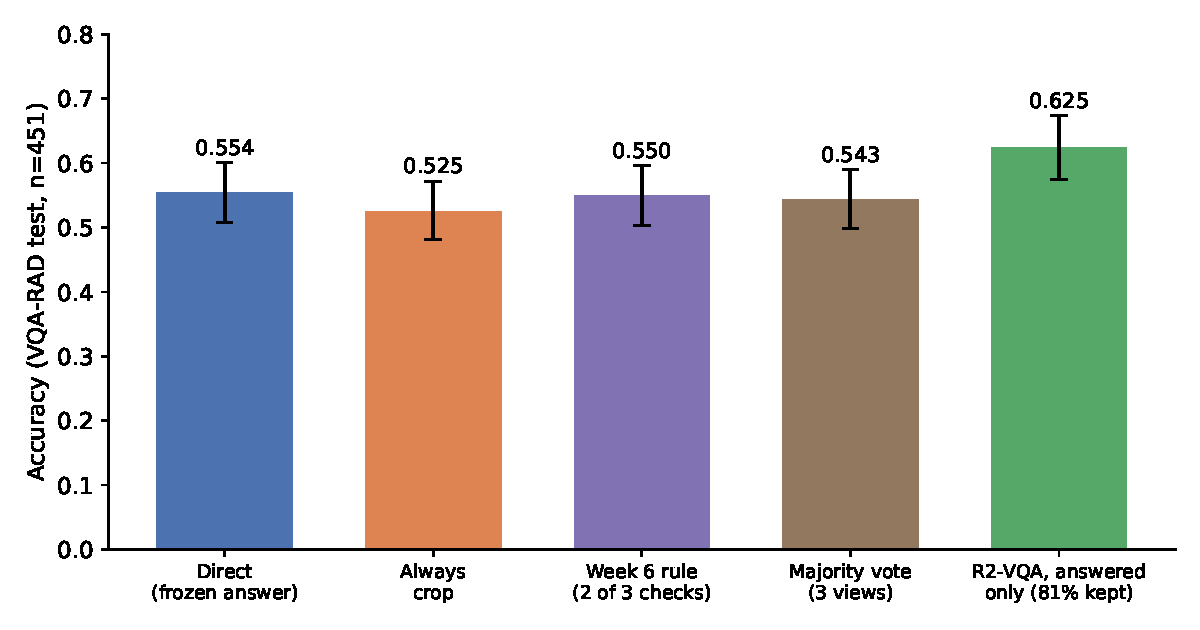
\includegraphics[width=0.85\linewidth]{figures/fig1_accuracy_bars.pdf}
\caption{Accuracy of the answer rules on the test split with 95\% CIs, and accuracy of R2-VQA on the questions it answers.}\label{fig:bars}
\end{figure}

\subsection{Abstaining on view agreement improves accuracy on answered questions}
At the frozen threshold, R2-VQA answers 80.9\% of test questions (development target 80.0\%) with accuracy 0.625 [0.575, 0.674], against 0.554 for answering everything. The gain is +0.070 [0.046, 0.095], an interval that excludes zero. Accuracy on the abstained questions is 0.256. Of all test questions, 14.2\% are wrong and withheld, 30.4\% are wrong and answered, and 4.9\% are right but withheld (Figure~\ref{fig:fail}).

\begin{figure}[t]\centering
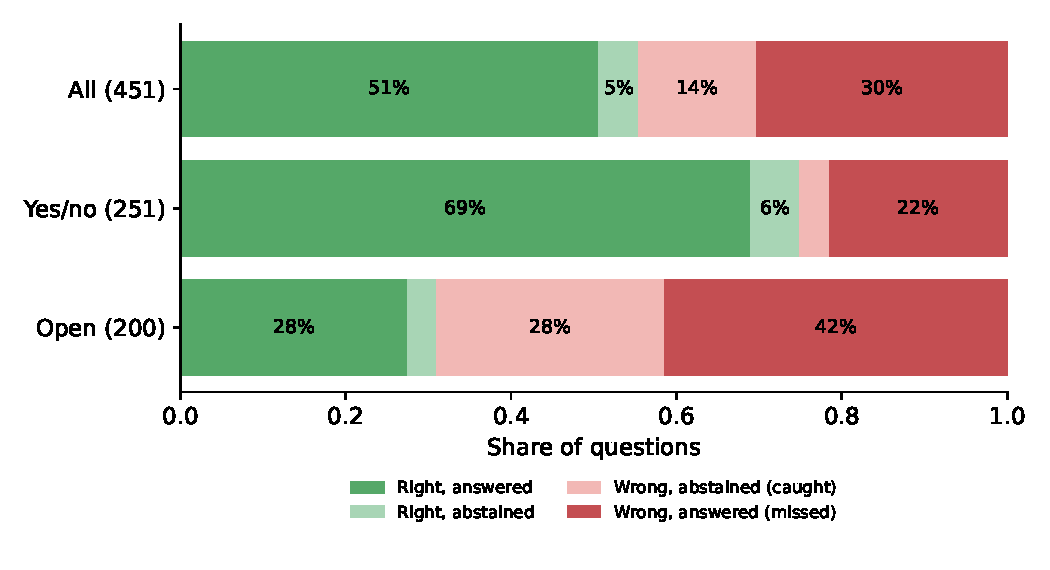
\includegraphics[width=0.85\linewidth]{figures/fig4_failure_categories.pdf}
\caption{Right and wrong answers, answered and abstained, at the frozen threshold, for all questions and by question type.}\label{fig:fail}
\end{figure}

\subsection{Comparison with plain confidence and simpler signals}
The R2-VQA score has higher AUROC than confidence (0.732 vs 0.666; difference +0.066, 95\% CI [0.028, 0.103], which excludes zero). At fixed coverage the difference is +0.019 at 80\% (CI [-0.008, 0.044], which includes zero) and +0.070 at 60\% (CI [0.026, 0.111], which excludes zero); these coverage-level comparisons are exploratory (Tables~\ref{tab:cov}, \ref{tab:vs}; Figure~\ref{fig:rc}). Simple agreement scores perform similarly to the fitted model in Table~\ref{tab:cov}, so we do not claim that the logistic regression is the best combination, only that view agreement carries information beyond confidence.

\begin{table}[t]
\centering\small
\caption{Accuracy when keeping the most reliable answers at fixed coverage, with 95\% bootstrap CIs. The first row uses the weights and threshold frozen on the development set.}\label{tab:cov}
\begin{tabular}{lcccc}
\toprule
Signal & Acc@100\% & Acc@80\% & Acc@60\% & Acc@40\% \\
\midrule
R2-VQA logistic signal (frozen weights) & 0.554 [0.508, 0.601] & 0.629 [0.576, 0.681] & 0.708 [0.646, 0.768] & 0.739 [0.672, 0.794] \\
confidence & 0.554 [0.508, 0.601] & 0.609 [0.562, 0.659] & 0.638 [0.579, 0.694] & 0.689 [0.611, 0.756] \\
consistency (3 views agree) & 0.554 [0.508, 0.601] & 0.634 [0.582, 0.684] & 0.683 [0.627, 0.742] & 0.722 [0.656, 0.789] \\
crop agrees with direct & 0.554 [0.508, 0.601] & 0.626 [0.573, 0.681] & 0.716 [0.661, 0.768] & 0.722 [0.661, 0.789] \\
\bottomrule
\end{tabular}
\end{table}

\begin{table}[t]
\centering\small
\caption{R2-VQA logistic signal minus plain confidence, paired bootstrap over test questions (2000 resamples). AUROC is the pre-specified comparison; the coverage-level rows are exploratory.}\label{tab:vs}
\begin{tabular}{lccc}
\toprule
Metric & Difference & 95\% CI & Share $>0$ \\
\midrule
Acc@80\% & 0.019 & [-0.008, 0.044] & 0.881 \\
Acc@60\% & 0.070 & [0.026, 0.111] & 0.999 \\
Acc@40\% & 0.050 & [-0.006, 0.106] & 0.949 \\
AUROC & 0.066 & [0.028, 0.103] & 1.000 \\
\bottomrule
\end{tabular}
\end{table}


\begin{figure}[t]\centering
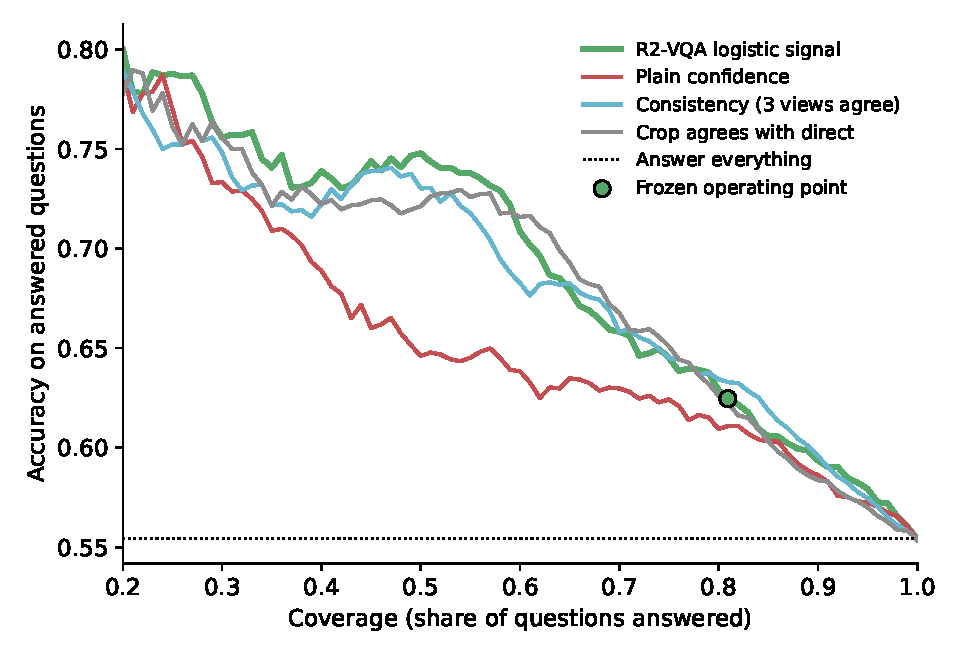
\includegraphics[width=0.7\linewidth]{figures/fig2_risk_coverage.pdf}
\caption{Risk--coverage curves on the test split. The marker is the frozen operating point.}\label{fig:rc}
\end{figure}

\subsection{Where the gain comes from}
Table~\ref{tab:type} breaks the results down by question type. Yes/no questions have direct accuracy 0.749 and are mostly answered (coverage 0.904), so abstention changes accuracy little (0.762 on answered). Open questions are much harder (direct accuracy 0.310); the model abstains on more of them (coverage 0.690) and accuracy on answered open questions is 0.399. In neither question type is the R2-VQA signal better than plain confidence (yes/no: 0.641 vs 0.662; open: 0.780 vs 0.788). The pooled AUROC advantage therefore partly reflects the signal separating harder from easier question types. Figure~\ref{fig:compute} shows accuracy against model calls per question.

\begin{table}[t]
\centering\small
\caption{Results by question type at the frozen threshold. AUROC columns compare the R2-VQA signal with plain confidence within each type.}\label{tab:type}
\begin{tabular}{lrrrrrr}
\toprule
Type & $n$ & Direct acc. & Coverage & Acc. answered & AUROC R2-VQA & AUROC conf. \\
\midrule
closed\_yes\_no & 251 & 0.749 & 0.904 & 0.762 & 0.641 & 0.662 \\
open & 200 & 0.310 & 0.690 & 0.399 & 0.780 & 0.788 \\
\bottomrule
\end{tabular}
\end{table}


\begin{figure}[t]\centering
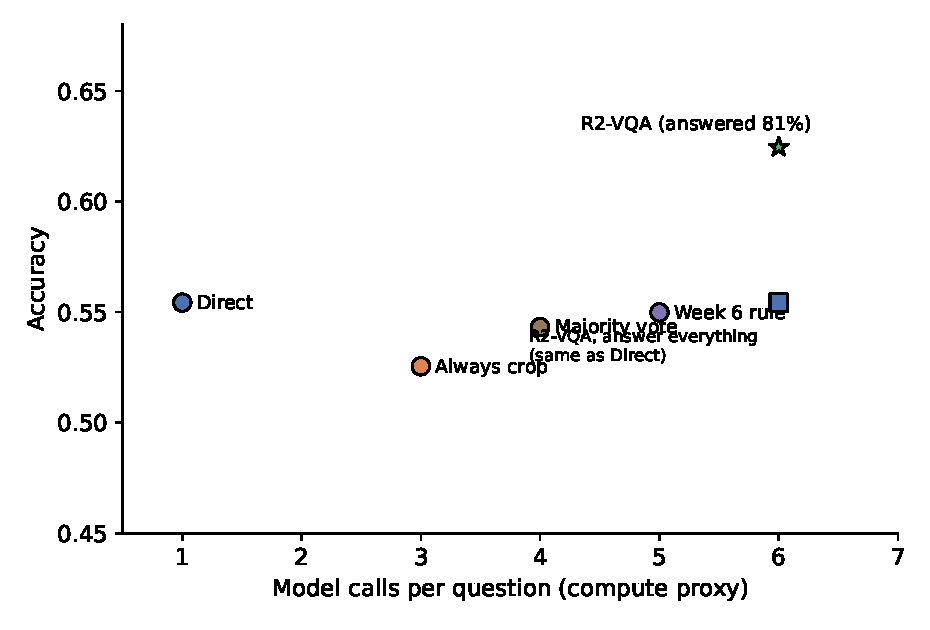
\includegraphics[width=0.7\linewidth]{figures/fig3_accuracy_vs_compute.pdf}
\caption{Accuracy against model calls per question (a compute proxy). The star is R2-VQA accuracy on the questions it answers.}\label{fig:compute}
\end{figure}

\section{Ablations and Negative Findings}
\paragraph{Region necessity.} The ``masking changes the answer'' feature was meant to indicate that the predicted region matters. On the development set its AUROC for predicting correctness was 0.438, below chance, and masking lowered accuracy to 0.410 (Table~\ref{tab:dev}). We therefore do not present it as evidence that the model's answer depends on the predicted region.
\paragraph{Development-set signal quality.} On the development set the logistic score reached AUROC 0.732 against 0.673 for confidence, which met the pre-set requirement of a gain of at least 0.02.
\paragraph{Baselines not run.} We did not run self-consistency sampling or tiling baselines in the final test run. \todo{run or remove from the claims.}

\section{Limitations}
\begin{itemize}
\item \textbf{The test split was not fresh.} 451 of 451 test questions (100.0\%) appear in result files from earlier exploratory weeks (Week 2: 100, Week 3: 100, Week 4: 100, Week 5: 131, Week 6: 451). The final method's weights, threshold and decision rules were fit only on 500 training-split questions, but earlier work on the test split influenced which views, prompt and signals were considered. A genuinely unseen evaluation set is needed to remove this concern.
\item \textbf{One dataset, one model, small $n$.} VQA-RAD is small and the test set has 451 questions; intervals are wide, and results may not transfer to other models or datasets.
\item \textbf{Strict string matching} undercounts correct open-ended answers that are phrased differently from the reference.
\item \textbf{Question-type effect.} The advantage over confidence is not present within question types, so it should not be read as better per-question reliability estimation.
\item \textbf{Modality labels} used in breakdowns were produced by the model itself and most questions fall in an ``other'' group; we do not draw conclusions from them.
\item \textbf{Compute.} The pipeline needs six model calls per question, and wall-clock cost was not measured per question.
\end{itemize}

\section{Conclusion}
Querying a vision-language model on several views of a medical image does not make its answers more accurate, but agreement between those views gives a training-free signal for withholding answers that improves accuracy on the answered questions. The benefit over plain confidence is real in ranking quality but modest at the operating point we froze, and it is tied to question difficulty. We hope the evaluation protocol, with decisions fixed before the test run and negative findings reported, is useful for similar studies.

\bibliographystyle{plain}
\todo{add references.bib and \texttt{\textbackslash bibliography\{references\}} once citations are added}
\end{document}
